%! Suppress = MissingImport
%! Suppress = TooLargeSection
%! Suppress = SentenceEndWithCapital
%! Suppress = LineBreak
%! Suppress = MissingLabel
%! Suppress = Unicode

\documentclass[main.tex]{subfiles}

\begin{document}

    \section{Metody dowodzenia poprawności pętli.}

    \textbf{Asercja} - warunek logiczny wyrażający zależności między zmiennymi
    algorytmu w kontekście ich aktualnego stanu.
    \begin{itemize}[noitemsep]
        \item \textbf{początkowa} - określa warunek wejściowy algorytmu.
        \item \textbf{końcowa} - określa wyniki algorytmu.
        \item Asercje początkowa i końcowa stanowią \textbf{specyfikację algorytmu}
    \end{itemize}

    \noindent \textbf{Algorytm A}:
    \begin{itemize}
        \item ma własność \textbf{określoności obliczeń} względem warunku $\alpha$, jeśli dla każdych danych
        spełniających warunek $\alpha$ działanie algorytmu A nie zostanie zerwane.

        \item ma \textbf{własność stopu} względem warunku $\alpha$, jeśli dla każdych danych spełniających warunek
        $\alpha$ działanie algorytmu A nie ciągnie się w nieskończoność (oznaczenie stop $( \alpha, A )$ ).

        \item jest \textbf{częściowo poprawny} względem warunku początkowego $\alpha$ i końcowego $\beta$,
        gdy dla każdych danych spełniających $\alpha$, \textbf{jeżeli} działanie algorytmu dochodzi do końca, wyniki
        spełniają $\beta$:
        \[cp ( \alpha, z \leftarrow w, \beta ) \iff ( \alpha \Rightarrow \beta|_{z \leftarrow w})\]

        \item jest \textbf{całkowicie} (semantycznie) \textbf{poprawny} względem warunku
        początkowego $\alpha$ i końcowego $\beta$, jeśli ma własność określoności obliczeń
        względem $\alpha$, ma własność stopu względem $\alpha$ oraz jest częściowo
        poprawny względem $\alpha$ i $\beta$:
        \[sp ( \alpha, A, \beta ) \iff obl ( \alpha, A ) \wedge stop ( \alpha, A ) \wedge cp ( \alpha, A, \beta )\]
    \end{itemize}


    \section{Odwrotna Notacja Polska: definicja, własności, zalety i wady, algorytmy.}

    \begin{itemize}[noitemsep]
        \item notacja postfiksowa,
        \item jednoznacznie wyznacza kolejność wykonywania działań,
        \item pozwala na całkowitą rezygnację z nawiasów.
        \item Zalety:
        \begin{itemize}
            \item ułatwione obliczenia na komputerze - wykorzystuje jedynie stos
            \item prosty algorytm konwersji między standardowym zapisem infiksowym a ONP
            wykorzystywany w wielu algorytmach wykorzystujących jako wejście zapis działań
            brak konieczności stosowania nawiasów
        \end{itemize}
        \item Wady:
        \begin{itemize}
            \item mniej czytelny dla człowieka (wymaga przyzwyczajenia)
            \item podczas zapisu na kartce ``12 34'' + może wyglądać jak ``123 4'' + (xD)
        \end{itemize}
    \end{itemize}

    \subsection{Algorytm obliczenia wartości wyrażenia ONP}
    Dla wszystkich symboli z wyrażenia ONP wykonuj:
    \begin{itemize}[noitemsep]
        \item jeśli symbol jest liczbą, to odłóż go na stos,
        \item jeśli symbol jest operatorem (funkcją):
        \begin{itemize}[noitemsep]
            \item zdejmij ze stosu oczekiwaną liczbę elementów (parametrów),
            \item odłóż na stos wynik działania operatora.
        \end{itemize}
    \end{itemize}
    Zdejmij ze stosu wynik.

    \subsection{Algorytm konwersji z notacji infiksowej do ONP}

    Wykonuj dopóki dane na wejściu.
    \begin{itemize}[noitemsep]
        \item Weź kolejny element z wejścia.
        \item Jeśli element jest operandem, to dopisz element na wyjście.
        \item Wpp (element jest operatorem, przecinkiem lub nawiasem):
        \begin{itemize}
            \item Jeśli element jest operatorem o1, to dopóki:
            \begin{itemize}
                \item lewa łączność(o1) i priorytet <= od operatora na stosie, lub
                \item prawa łączność(o1) i priorytet < od operatora na stosie
            \end{itemize}
            wstaw o1 na wyjście.
            \item Lub jeśli element == '(' to wstaw element na stos.
            \item Lub jeśli element == ')' to przepisz elementy ze stosu na wyjście aż do '(', nawias usuń.
        \end{itemize}
    \end{itemize}
    Przepisz elementy ze stosu na wyjście.


    \section{Modele obliczeń: maszyna Turinga.}

    \begin{definition}
        \textbf{Formalna definicja maszyny Turinga}. Maszynę Turinga opisujemy poprzez krotkę:
        \[MT ~ = ~<Q, \Sigma, \delta, \tau, q_0, B, F >\]
        gdzie:
        \begin{itemize}[noitemsep]
            \item $Q$ - skończony zbiór stanów,
            \item $q_0 \in Q$ - stan początkowy,
            \item $F \subset Q$ - zbiór stanów końcowych,
            \item $\tau$  - skończony zbiór dopuszczalnych symboli,
            \item $b \in \tau$  - symbol pusty,
            \item $\Sigma \subset \tau \ \{b\} $ - zbiór symboli wiejściowych,
            \item $\delta$ - funkcja sterująca.
            \begin{itemize}[noitemsep]
                \item W wersji niedeterministycznej postaci maszyny Turinga:
                \[ \delta \subset (Q \times \tau)  \times (\tau \times \{\leftarrow, \rightarrow, \downarrow\}  \times Q)\]
                \item W wersji deterministycznej:
                \[ \delta : Q \times \tau \mapsto \tau \times \{\leftarrow, \rightarrow, \downarrow\} \times Q\]
            \end{itemize}
        \end{itemize}

        \textbf{Tablica sterująca} to dwuwymiarowa tablica indeksowana: stanami w jednym wymiarze, a symbolami taśmy w
        drugim. Elementy tablicy zawierają trójki działania maszyny, czyli wartości funkcji sterowania $\delta$.
    \end{definition}


    \section{Modele obliczen: automat skończony, automat ze stosem.}
    \subsection{Automat skończony deterministyczny}
    \begin{definition}
        \textbf{Automat skończony deterministyczny} oznaczamy piątką parametrów:
        \[\mathcal{A} = (S, A, f, s_{0}, T)\]
        S -- zbiór stanów, A - alfabet, T $\in$ S -- zbiór terminali, $s_{0} \in$ S -- stan początkowy\\
        $f: S\times A \rightarrow$-- funkcja przejścia S \\

        Każdy język skończony jest akceptowany przez pewien deterministyczny automat skończony.
    \end{definition}

    \begin{definition}
        Automaty $\mathcal{A}_{1}$ i  $\mathcal{A}_{2}$ są \textbf{równoważne}, jeżeli rozpoznają ten sam język, czyli:
        \[L(\mathcal{A}_{1}) = L(\mathcal{A}_{2})\]
    \end{definition}

    \begin{definition}
        Każdy automat $\mathcal{A}$ = (S, A, f, $s_{0}$, T) wyznacza w wolnym monoidzie $A^{*}$ \textbf{prawą kongruencję
        automatową} okresloną w następujący sposób:
        \[\forall u,v \in A^{*}, u \sim_\mathcal{A} v \Leftrightarrow f(s_{0}, u) = f(s_{0}, v)\]

        Automat ilorazowy to automat, w którym stanami są klasy równoważności.
    \end{definition}

    \begin{definition}
        $L \subset  A^{*}$ język, $u \in A^{*}$ słowo.
        \textbf{Pochodną Brzozowskiego (residuum)} z języka L względem słowa u nazywamy język
        \[u^{-1}L = \{w \in A^{*}  : uw \in L \}\]
    \end{definition}

    \begin{definition}
        Monoidem przejśc automatu $\mathcal{A}$ nazywamy monoid:
        \[\mathcal{M(A)} = \tau_\mathcal{A}(A^*) \subset S^{S} = \{tau_\mathcal{A}(a) : a \in A^*\}\]
        bedący zbiorem generatorów (unikalnych reprezentacji) automatu $\mathcal{A}$.
    \end{definition}

    \subsection{Automat skończony niedeterministyczny}
    \begin{definition}
        \textbf{Automat skończony niedeterministyczny} różni funkcja przejścia f zdefiniowana:
        \[f : S \times A \rightarrow \mathcal{P} (S) \]

        Słowo x jest akceptowane gdy $f^{*}$($S_{0}$, x) $\cap$ T $\neq \emptyset$
    \end{definition}

    \subsection{Automat ze stosem}
    \begin{definition}
        \textbf{Automat ze stosem} to
        \[\mathcal{AS} = (A, A_{S}, Q, f, s_{0}, z_{0}, Q_{F})\]
        A -- alfabet, $A_{S}$ -- alfabet stosu, Q -- zbiór stanów,\\
        $Q_{F} \subset Q$ -- zbiór stanów końcowych\\
        $q_{0} \in Q$ -- stan początkowy, $z_{0} \in A_{S}$ -- symbol początkowy stosu\\
        f: $A_{s} \times Q \times (A \cup \{1\}) \rightarrow \mathcal{P}_{sk}(A^{*}_{S} \times Q)$ -- funkcja przejść
    \end{definition}


    \section{Złożoność obliczeniowa - definicja notacji: $O, \Omega, \Theta$.}
    \begin{definition}
        Niech$f, g, h: \mathbb{N} \rightarrow \mathbb{R}_{+} \cup \{0\}$, wtedy:
        \begin{itemize}
            \item $\mathbf{f(n) = O(g(n))}$ -- f jest \textbf{co najwyżej rzędu} g, gdy
            \[\exists c > 0, n_0 \in \mathbb{N} \forall n \geq n_0 f(n) \leq cg(n).\]
            \item $\mathbf{f(n) = \Omega(g(n))}$ -- f jest \textbf{co najmniej rzędu} g, gdy
            \[g(n) = O(f(n)).\]
            \item $\mathbf{f(n) = \Theta(g(n))}$ -- f jest \textbf{dokładnie rzędu} g, gdy
            \[f(n) = O(g(n)) \wedge  f(n) = \Omega(g(n)).\]
        \end{itemize}
    \end{definition}


    \section{Złożoność obliczeniowa - pesymistyczna i średnia.}

    \begin{definition}
        Niech:\\
        $D_n$ - zbiór danych rozmiaru n,\\
        $t(d)$ - liczba operacji dominujących,\\
        $X_n$ - zmienna losowa dla $t(d) \in D_n$,\\
        $p_{kn}$ - rozkład prawdopodbieńdstwa zmiennej $X_n$.

        \textbf{Optymistyczna złożoność czasowa}:
        \[Opt(n) = inf\{t(d) : d \in D_n\}\]

        \textbf{Średnia złożoność czasowa}:
        \[A(n) = ave(X_n) = \sum_{k \geq 0}kp_{nk}\]

        \textbf{Pesymistyczna złożoność czasowa}:
        \[W(n) = sup\{t(d) : d \in D_n\}\]
    \end{definition}

    \begin{definition}
        \textbf{Koszt amortyzowany} to \textbf{średni czas} wykonania przypadający na jedną operację w pesymistycznym
        ciągu operacji. Koszt amortyzowany różni się od kosztu średniego tym, że bierze pod uwagę pesymistyczny ciąg
        operacji i nie jest metodą probabilistyczną.
    \end{definition}


    \section{Metoda "dziel i zwyciężaj": zalety i wady.}

    \begin{enumerate}[noitemsep]
        \item \textbf{Dziel} problem na mniejsze podproblemy, aż do przypadków bazowych.
        \item \textbf{Zwyciężaj} rozwiązując przypadki bazowe.
        \item \textbf{Łącz} wyniki otrzymane z podproblemów.
    \end{enumerate}

    \subsection{Zalety}

    \begin{itemize}
        \item Optymalne użycie pamięci podręcznej (\textit{cache}): problemy dostatecznie małe
        rozwiązywane są w pamięci nieprzekraczającej wielkości pamięci podręcznej.

        \item Znacząco lepsza złożoność obliczeniowa od bardziej prymitywnych podejść.
    \end{itemize}

    \subsection{Wady}

    \begin{itemize}
        \item Rekurencja nieliniowa - przekształcenie w algorytm iteracyjny jest nietrywialne (w szczególności nie
        zostanie to wykonane przez kompilator).

        \item Potencjalnie wysoka złożoność pamięciowa algorytmu rekurencyjnego / iteracyjnego ze stosem.
        Ponadto rozmiar stosu może przekroczyć pamięć komputera.

        \item Możliwość wielokrotnego rozwiązywania identycznych problemów (programowanie dynamiczne, memoization)/
    \end{itemize}


    \section{Lista: ujęcie abstrakcyjne, możliwe implementacje i ich złożoności.}
    \begin{definition}
        Lista jest abstrakcyjną strukturą danych (ADT), która posiada następujące właściwości
        \begin{itemize}[noitemsep]
            \item Przechowuje elementy \textbf{tego samego typu}
            \item Dostęp do danych jest \textbf{sekwencyjny}
            \item Elementy w liście są \textbf{liniowo uporządkowane}
            \item W sensie matematycznym lista jest skończonym ciągiem elementów ustalonego typu.
        \end{itemize}
    \end{definition}

    Wyróżnia się dwa podstawowe sposoby implementacji listy:
    \begin{itemize}
        \item \textbf{Tablica} - wykorzystuje pamięć w sposób \textbf{statyczny}, posiada zmienne wskazujące na jej
        maksymalny rozmiar, ilość zajętych miejsc.

        \item \textbf{Lista wiązana}:
        \begin{enumerate}
            \item Lista wiązana \textbf{jednokierunkowa} -- z każdego elementu możliwe jest przejście do jego następnika.
            \item Lista wiązana \textbf{dwukierunkowa} -- z każdego elementu możliwe jest przejście do jego następnika
            lub poprzednika.
            \item Lista \textbf{z głową}, \textbf{cykliczna} itd.
        \end{enumerate}
    \end{itemize}


    \section{Kolejka i kolejka priorytetowa: ujęcie abstrakcyjne, możliwe implementacje i ich złożoności.}
    \subsection{Kolejka}
    \begin{definition}
        \textbf{Kolejka FIFO} (First In First Out) to lista, w której:
        \begin{itemize}[noitemsep]
            \item Wstawianie nowego elementu odbyca się na końcu kolejki \textbf{rear}.
            \item Usuwanie elementu odbywa się na początku kolejki \textbf{front}.
            \item Wyróżnia się dwa podstawowe sposoby implementacji kolejki:
            \begin{itemize}
                \item Tablica cykliczna,
                \item Lista wiązana.
            \end{itemize}
            \item Wszystkie operacj w czasie stałym.
        \end{itemize}
    \end{definition}


    \subsection{Kolejka Priorytetowa}
    \begin{definition}
        Kolejka Priorytetowa to lista, w której:
        \begin{itemize}
            \item Usuwany jest zawsze element o największej (najmniejszej) wartości.
            \item Wyróżnia się trzy podstawowe sposoby implementacji kolejki priorytetowej:
            \begin{itemize}
                \item Kopiec Max (Min)
                \item Lista/Tablica Nieuporządkowana - NIEEFEKTYWNE!
                \item Lista/Tablica Uporządkowana Rosnąco (Malejąco) - NIEEFEKTYWNE!
            \end{itemize}
        \end{itemize}
    \end{definition}


    \section{Algorytmy sortowania QuickSort i MergeSort: metody wyboru pivota w QS; złożoności.}

    \subsection{QuickSort.}

    \begin{minted}{python}
        def quickSort(arr, start, end):
        if (start < end):
        pivot = partition(arr, start, end)
        quickSort(arr, start, pivot - 1)
        quickSort(arr, pivot + 1, end)


        def partition (arr, start, end):
        pivot = arr[end]
        i = (start - 1)

        for j in range [start,end- 1]:
        if (arr[j] < pivot):
        i++;
        swap arr[i] and arr[j]

        swap arr[i + 1] and arr[end])
        return (i + 1)
    \end{minted}
    \textbf{Złożoność}: pesymistyczna - $O(n^2)$, średnia i optymistyczna - $O(nlog_2 n)$.

    \noindent \textbf{Sposoby wybrania pivota}: pierwszy, ostatni lub losowy element; \textbf{mediana} z pierwszego,
    środkowego i ostatniego

    \subsubsection{MergeSort.}

    \begin{minted}{python}
        def mergeSort (arr, start, end):
        if end > start:
        middle = (start+end)/2

        mergeSort (arr, start, middle)
        mergeSort (arr, middle+1, end)

        merge (arr, start, middle, right)
    \end{minted}
    \textbf{Złożoność:} pesymistyczna, średnia, optymistyczna - $O(nlogn)$.


    \section{Algorytm sortowania bez porównań (sortowanie przez zliczanie, sortowanie kubełkowe oraz sortowanie pozycyjne).}

    \subsection{CountSort.}
    \begin{minted}{python}
        def countSort (arr):
        count = []
        for a in arr:
        count[a] += 1

        i = 0;
        for j in range [0, arr.len]:
        while (count[i] == 0):
        i++
        arr[j] = i
        count[i]--
    \end{minted}
    \textbf{Złożoność:} $O(n+k)$.

    \subsection{BucketSort.}
    \begin{minted}{python}
        bucketSort (arr):
        n = arr.len
        buckets = [{} for i in range [1,n]]

        for a in arr:
        buckets[n*arr[i]].add(arr[i])

        for b in buckets:
        sort(b)

        i = 0
        for b in buckets:
        for a in b:
        arr[i++] = a
    \end{minted}
    \textbf{Złożoność:} pesymistyczna -  $O(n^2)$, średnia - $O\left(n + \frac{n^2}{k} + k\right)$.

    \subsection{RadixSort.}
    \begin{minted}{python}
        def radixSort (arr):
        for all digits ascending:
        countSort(arr, digit)
    \end{minted}
    \textbf{Złożoność:} $O(d(n+k))$, gdzie d jest liczbą cyfr.


    \section{Reprezentacja drzewa binarnego za pomocą porządków (preorder, inorder, postorder).}

    \begin{minted}{python}
        def preorder (v):
        func(v)
        preorder(v.left)
        preorder(v.right)

        def inorder (v):
        inorder(v.left)
        func(v)
        inorder(v.right)

        def postorder (v):
        postorder(v.left)
        postorder(v.right)
        func(v)
    \end{minted}

    Możemy odtworzyć wyjściowe drzewo, jeśli mamy inorder i post- lub pre-order.


    \section{Algorytmy wyszukiwania następnika i poprzednika w drzewach BST; usuwanie węzła.}

    \begin{definition}
        \textbf{Binarne drzewo poszukiwań (BST)} - dynamiczna struktura danych będąca drzewem binarnym, w którym lewe
        poddrzewo każdego węzła zawiera wyłącznie elementy o kluczach mniejszych niż klucz węzła a prawe poddrzewo
        zawiera wyłącznie elementy o kluczach nie mniejszych niż klucz węzła.
    \end{definition}

    \subsection{Wyszukiwanie następnika i poprzednika w BST.}
    \begin{definition}
        \textbf{Następnik} danego węzła to węzeł, który jest odwiedzany jako \textbf{następny} w przypadku przechodzenia drzewa
        metodą \textbf{inorder}. Sposób wyznaczenia nie wymaga porównywania żadnych kluczy, jest to w praktyce:
        \begin{itemize}[noitemsep]
            \item skrajnie lewy element prawego poddrzewa węzła, jeśli istnieje; wpp
            \item pierwszy napotkany przodek węzła, dla którego węzeł jest w lewym poddrzewie.
        \end{itemize}
    \end{definition}

    \begin{definition}
        \textbf{Poprzednik} danego węzła to węzeł, który jest odwiedzany jako \textbf{poprzedni} w przypadku przechodzenia drzewa
        metodą \textbf{inorder}. Sposób wyznaczenia nie wymaga porównywania żadnych kluczy, jest to w praktyce:
        \begin{itemize}[noitemsep]
            \item skrajnie prawy element lewego poddrzewa węzła, jeśli istnieje; wpp
            \item pierwszy napotkany przodek węzła, dla którego węzeł jest w prawym poddrzewie.
        \end{itemize}
    \end{definition}

    \subsection{Usuwanie węzła z BST.}

    \begin{theorem}
        \textbf{Usuwanie} węzła z BST w trzech przypadkach:
        \begin{enumerate}[noitemsep]
            \item usuwany węzeł jest \textbf{liściem} -- \textbf{usuwamy},
            \item usuwany węzeł ma \textbf{jednego} syna -- podstawiamy \textbf{syna},
            \item usuwany węzeł ma \textbf{dwóch} synów -- podstawiamy jego \textbf{następnik}.
        \end{enumerate}
    \end{theorem}


    \section{B-drzewa: operacje i ich złożoność.}
    \begin{itemize}
        \item B-drzewa to \textbf{rozszerzone drzewa BST zoptymalizowane pod kątem operacji wejścia/wyjścia}.

        \item Mają ustalony \textbf{rząd}. B-drzewo rzędu K musi spełniać poniższe warunki:
        \begin{itemize}
            \item Korzeń jest liściem lub ma od 2 do K synów
            \item Wszystkie liście są na tym samym poziomie $\rightarrow$ wysokość $\in [\log_{\frac{K}{2}} \frac{n}{\frac{K}{2}}, \log_{K} \frac{n}{K}]$
            \item Każdy węzeł wewnętrzny (oprócz korzenia) ma $s \in [\lceil K/2 \rceil, K]$ synów i $s-1$ kluczy (wartości)
        \end{itemize}

        \item \textbf{Złożoność} wszystkich operacji na B-drzewach -- $O(K \log_{K} n)$.
        \begin{itemize}
            \item wyszukiwanie -- podobne jak w BST, do przeszukiwania węzłów używamy binsearcha
            \item wstawianie -- wyszukujemy odpowiedni liść i do niego wstawiamy; jeśli się przepełni ($\geq K$), to
            jedną z wartości wstawiamy do rodzica a pozostałe dzielimy na dwa nowe liście (rekurencja)
            \item usuwanie -- znajdujemy żądany element, zastępujemy największym mniejszym lub najmniejszym większym
            i równoważymy drzewo
        \end{itemize}

        \item Odmianą B-drzew są \textbf{drzewa B+} -- wszystkie wartości trzymane są w liściach, liście powiązane w listę.

    \end{itemize}

    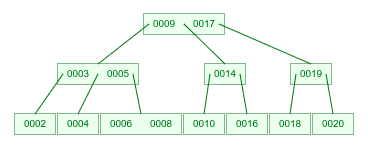
\includegraphics[]{b-trees/b-tree-example.png}


    \section{Drzewa AVL: rotacje, operacje z wykorzystaniem rotacji i ich złożoność.}

    \begin{itemize}
        \item odmiana drzew BST, w której \textbf{różnica między wysokością prawego i lewego poddrzewa} danego węzła
        wynosi \textbf{maksymalnie 1}.
        \item Operacje wyszukiwania, wstawiania oraz usuwania mają \textbf{złożoność} $O(\log_{2} n)$.
    \end{itemize}

    \subsection{Rotacje}
    \begin{multicols}{2}
        \textbf{Rotacja RR} \\

        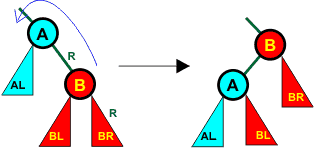
\includegraphics[width=0.8\linewidth]{avl-trees/rr-rotation.png}
        \columnbreak \\
        \textbf{Rotacja LL} \\

        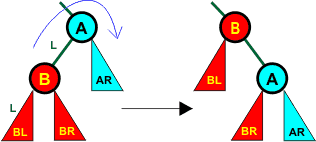
\includegraphics[width=0.8\linewidth]{avl-trees/ll-rotation.png}
    \end{multicols}

    \begin{itemize}
        \item \textbf{Rotacja RR} -- gdy dla węzła A prawe poddrzewo z korzeniem B zaburza równowagę, ale samo
        poddrzewo B jest zrównoważone ("pojedyncza nierównowaga na prawo"),
        \item \textbf{Rotacja LL} -- analogicznie dla lewego poddrzewa ("pojedyncza nierównowaga na prawo"),
        \item  \textbf{Rotacja RL} (LL $\rightarrow$ RR) -- prawe poddrzewo B niezrównoważone przez jego
        lewe poddrzewo C ("podwójna nierównowaga prawo-lewo),
        \item \textbf{Rotacja LR} (RR $\rightarrow$ LL) -- lewe poddrzewo B niezrównoważone przez jego prawe
        poddrzewo C ("podwójna nierównowaga lewo-prawo").
    \end{itemize}


    \section{Algorytmy przeszukiwania wszerz i w głąb w grafach.}

    Przejście przez wszystkie \textbf{osiągalne} z wierzchołka startowego $s$ wierzchołki grafu $G$.
    \begin{itemize}[noitemsep]
        \item \textbf{złożoność obliczeniowa} -- $\theta(e + v)$
        \item złożoność \textbf{pamięciowa} --  $\theta(v)$
    \end{itemize}

    \subsection{Przeszukiwanie grafu wszerz (\textit{breadth first search}, BFS)}

    \noindent \textbf{Algorytm}\\
    Dopóki \textbf{kolejka} nie jest pusta:
    \begin{enumerate}[noitemsep]
        \item Zdejmij $x$ z kolejki
        \item Pomaluj $x$ na czarno
        \item Dla każdego niepomalowanego na czarno $v$, sąsiadującego z $x$ wrzuć
        $v$ do kolejki
    \end{enumerate}

    \subsubsection{Cechy}

    \begin{itemize}[noitemsep]
        \item \textbf{Kompletność}: BFS dla \textbf{nieskończonego grafu} zwróci wszystkie poprawne
        odpowiedzi, w przeciwieństwie do DFS.

        \item \textbf{Zastosowania}:
        \begin{itemize}[noitemsep]
            \item Najkrótsza droga do $s$
            \item Wykrywanie cykli grafu nieskierowanego
            \item Sprawdzanie dwudzielności grafu
            \item Algorytmy sieci przepływowych
            \item Garbage collection
        \end{itemize}
    \end{itemize}

    \subsection{Przeszukiwanie grafu wgłąb (\textit{depth first search}, DFS)}

    \noindent \textbf{Algorytm}\\
    Dla danego wierzchołka $x$ (zaczynając od $s$):
    \begin{enumerate}[noitemsep]
        \item Pomaluj $x$ na czarno
        \item Wywołaj się rekurencyjnie (odłóż $x$ na \textbf{stos}) dla każdego niepomalowanego na czarno $v$,
        sąsiadującego z $x$
    \end{enumerate}


    \subsubsection{Cechy}

    \begin{itemize}[noitemsep]
        \item \textbf{Niekompletność} dla grafów \textbf{nieskończonych}
        \item \textbf{Zastosowania}
        \begin{itemize}[noitemsep]
            \item Minimalne drzewo rozpinające (dla grafów nieważonych)
            \item Wykrywanie cykli w grafie skierowanym/nieskierowanym
            \item Sortowanie topologiczne
            \item Algorytmy sieci przepływowych
            \item Garbage collection
        \end{itemize}
    \end{itemize}


    \section{Algorytmy wyszukiwania najkrótszej ścieżki (Dijkstry oraz Bellmana-Forda).}
    Algorytmy pozwalające na wyliczenie najkrótszych ścieżek od wierzchołka startowego $s$.\\

    \noindent \textbf{Funkcja relaksująca} sprawdza, czy ścieżka z $u$ do $w$ przez $v$ jest krótsza od aktualnie
    najkrótszej ścieżki.
    \\~\\
    \textit{relax(u, v, w)}:
    \vskip 0pt Jeśli $D[u, w] > D[u, v] + D[v, w]$ to:\\
    \hspace*{1cm} $D[u, w] = D[u, v] + D[v, w]$\\
    \hspace*{1cm} $P[u, w] = v$\\

    \subsection{Algorytm Dijkstry}

    \begin{itemize}[noitemsep]
        \item Algorytm zachłanny
        \item Nie działa poprawnie dla grafów z wagami ujemnymi
        \item \textbf{Złożoność}:
        \begin{itemize}[noitemsep]
            \item Implementacja tablicowa -- $O(|V|^2)$
            \item Implementacja z kopcem binarnym -- $O(|E|\log(|V|))$
        \end{itemize}
    \end{itemize}

    \noindent \textbf{Algorytm}\\

    \noindent $P = \{\}$ -- słownik wierzchołek : rodzic\\
    $D$ -- słownik odległości od $s$\\
    $S = \{v \in V : D[v]\}$ -- kolejka priorytetowa nieodwiedzonych wierzchołków względem ich odległości.\\
    $D[s] = 0; D[v] = \infty \; \forall v \in V \setminus \{s\}$.\\

    \noindent Dopóki $S$ niepusta:
    \begin{enumerate}[noitemsep]
        \item Usuń wierzchołek $v$ o najmniejszej wartości z $S$
        \item Dla każdego wierzchołka $w$ sąsiadującego z $v$ wywołaj \textit{relax(s, v, w)}
    \end{enumerate}

    \subsection{Algorytm Bellmana-Forda}

    \begin{itemize}[noitemsep]
        \item Działa poprawnie dla grafów z wagami ujemnymi (bez cykli o wagach ujemnych)
        \item Pozwala decydować, czy graf ma cykle ujemne
        \item Używany w protokole RIP
        \item Algorytm można zoptymalizować: jeśli w danej iteracji nie dokonał zmiany,
        należy przerwać jego działanie (ścieżki już są najkrótsze)
        \item \textbf{Złożoność} -- $O(|V| \cdot |E|)$
    \end{itemize}

    \noindent \textbf{Algorytm}\\

    \noindent $P = \{\}$ -- słownik wierzchołek : rodzic\\
    $D$ -- słownik odległości od $s$\\
    $D[s] = 0; D[v] = \infty \; \forall v \in V \setminus \{s\}$.\\

    Dla każdego wierzchołka w $V \setminus \{s\}$:
    \vskip 0pt Wywołaj \textit{relax(s, u, v)} dla każdej krawędzi $(u, v) \in E$
    \[\]

    Na koniec można wykonać sprawdzenie, czy w grafie nie ma cykli o wadze ujemnej:
    \[ \forall (u,v) \in E: ~~ D[v] > D[u] + e_{u \rightarrow v} \Rightarrow \text{istnieje cykl o wadze ujemnej}\]


    \subsection{Algorytm Floyda-Warshalla}

    Pozwala wyliczyć najkrósze ścieżki pomiędzy wszystkimi wierzchołkami w grafie $G$ (nieposiadającym ujemnych cykli).
    Inicjujemy słownik odległości jak poniżej:

    $D[(u, w) : u, w \in V] =
    \begin{cases}
        0, &\text{ jeśli } u = w\\
        e_{u \rightarrow w}, &\text{ jeśli } (u, w) \in E\\
        \infty, &\text{ jeśli } (u, w) \notin E
    \end{cases}$.

    \noindent I wywołujemy \textit{relax(u, v, w)} dla każdej trójki $(u, v, w) : u, w, v \in V$.
    \textbf{Złożoność} -- $\theta(v^3)$.

    \subsubsection{Cechy}
    \begin{itemize}[noitemsep]
        \item Prostota
        \item Pozwala obliczyć za jednym razem wszystkie ścieżki pomiędzy wierzchołkami
        \item Działa dla grafów z krawędziami ujemnymi (ale nie z cyklami ujemnymi)
        \item Złożoność jest niezależna od gęstości grafu
    \end{itemize}

    \newpage


    \section{Programowanie dynamiczne: podział na podproblemy, porównanie z metodą "dziel i zwyciężaj".}

    \textbf{Programowanie dynamiczne}:
    \begin{itemize}[noitemsep]
        \item Podział problemu na mniejsze podproblemy,
        \item Wyniki obliczeń zapisywane w tabeli (brak redundantnych obliczeń)
        \item Niejednokrotnie stosowanie techniki programowania dynamicznego daje w rezultacie algorytm
        \textbf{pseudowielomianowy}.
        \item \textbf{Metody programowania dynamicznego}:
        \begin{itemize}
            \item Metoda \textbf{zstępująca} z zapamiętywaniem polega na \textbf{rekurencyjnym wywoływaniu} funkcji z
            \textbf{zapamiętywaniem} wyników.
            \item Metoda \textbf{wstępująca} polega na rozwiązywaniu \textbf{wszystkich możliwych podproblemów},
            zaczynając od tych o najmniejszym rozmiarze; nie ma stosu wywołań.
        \end{itemize}
        \item \textbf{Zastosowanie} przy problemach typu:
        \begin{itemize}[noitemsep]
            \item Problem posiada powtarzające się podproblemy
            \item Podproblemy musi cechować \textbf{własność optymalnej podstruktury} -- optymalne rozwiązanie problemu
            jest funkcją optymalnych rozwiązań podproblemów.
            \item Zastosowanie brute force prowadzi do \textbf{ponadwielomianowej} liczby rozwiązań podproblemów,
            podczas gdy sama liczba różnych podproblemów jest wielomianowa.
        \end{itemize}
    \end{itemize}


    \section{Algorytm zachłanny: przykład optymalnego i nieoptymalnego wykorzystania.}

    \textbf{Algorytmy zachłanne} w każdym kroku podejmują taką decyzję, która w danej chwili jest najkorzystniejsza
    (\textbf{lokalnie optymalna}) licząc, że doprowadzi to do znalezienia rozwiązania \textbf{globalnie optymalnego}.

    \begin{itemize}[noitemsep]
        \item Nie zawsze znajdują rozwiązanie optymalne
        \item Są podzbiorem algorytmów \textbf{heurystycznych}
        \item Są to algorytmy \textbf{deterministyczne} – nie ma w nich losowości
    \end{itemize}

    Przykład - Pakowanie plecaka

    \begin{verbatim}
        posortuj nierosnąco przedmioty według wartości c[j]/w[j]
        aktualna_waga:=0

        for i:=1 to n do
        if w[i] + aktualna_waga <= W then
        dodaj i-ty przedmiot do plecaka
        aktualna_waga := aktualna_waga + w[i]
    \end{verbatim}

    Dane wejściowe, dla których algorytm będzie działał

    \begin{table}[H]
        \begin{center}
            \begin{tabular}{| p{5cm} | p{5cm}  | p{5cm}|}
                \hline
                &\multicolumn{2}{c|}{Działanie}\\
                &optymalne & nieoptymalne\\
                \hline
                \hline
                Pojemność & 8 & 7\\
                \hline
                Dane wejściowe & 5, 3, 2, 1, 1, 1 & 3, 3, 2, 2\\
                \hline
                Rozwiązanie & 5 + 3 + 2 :) & 3 + 3 = 6 :( \vskip 0mm optymalne: 3 + 2 + 2 = 7\\
                \hline
            \end{tabular}
        \end{center}
    \end{table}


    \section{Kolorowania wierzchołkowe (grafów planarnych) i krawędziowe grafów, algorytmy i ich złożoności.}

    \subsection{Kolorowanie grafów}
    \begin{itemize}
        \item Klasyczny roblem kolorowania (krawędziowego i wierzchołkowego) jest \textbf{NP-trudny} – nie istnieją
        wielomianowe algorytmy kolorujące grafy zawsze w sposób optymalny.
    \end{itemize}

    \noindent Przykładowy \textbf{algorytm kolorowania krawędziowego}:
    \begin{enumerate}[noitemsep]
        \item Użyj BFS do poruszania się po grafie.
        \item Wybierz wierzchołek i nadaj różne kolory jego krawędziom.
        \item Przejdź do kolejnego wierzchołka.
        \item Powtarzaj aż wszyskie krawędzie zostaną pokolorowane.
    \end{enumerate}

    \noindent \textbf{Algorytmy kolorowania wierzchołkowego}:
    \begin{itemize}
        \item \textbf{Algorytm SL} (smallest last):
        \begin{enumerate}[noitemsep]
            \item Znajdź wierzchołek o minimalnym stopniu i usuń go z grafu.
            \item Powtarzaj krok pierwszy tak długo, aż graf będzie pusty (zapamiętaj kolejność usuwanych wierzchołków).
            \item Koloruj wierzchołki zachłannie, zgodnie z ustaloną wcześniej kolejnością (zaczynając od wierzchołków usuniętych później).
        \end{enumerate}
        Algorytm SL jest \textbf{statyczny}, \textbf{złożoność} - $O(|V|+|E|)$.

        \item \textbf{Algorytm SLF} (saturated largest first)\\
        dopóki istnieją niepokolorowane wierzchołki wykonuj operacje:
        \begin{enumerate}[noitemsep]
            \item znajdź wierzchołek o maksymalnym stopniu spośród wierzchołków o maksymalnym stopniu nasycenia
            (liczbie kolorów sąsiadów)
            \item pokoloruj znaleziony wierzchołek zachłannie
        \end{enumerate}
        \textbf{Złożoność} algorytmu SLF wynosi $O(|E|\log |V|)$.
    \end{itemize}


    \subsection{Kolorowanie wierzchołkowe grafów planarnych}

    \begin{theorem}
        Liczba chromatyczna grafu planarnego jest równa lub mniejsza niż 4
    \end{theorem}

    \textbf{Każdy graf planarny można pokolorować 5 kolorami w czasie liniowym}.

    %TODO - coś więcej o tych grafach?


    \section{Algorytmy wyszukiwania minimalnego drzewa rozpinającego: Boruvki, Prima i Kruskala.}

    \textbf{Algorytm Boruvki} - $O(ElogV)$.
    \begin{enumerate}[noitemsep]
        \item Weź wszystkie wierzchołki, ale bez krawędzi - każdy wierzchołek jest osobnym drzewem.
        \item Dla każdego drzewa znajdź krawędź o najmniejszej wadze w oryignalnym grafie, która łączy je z innym drzewem.
        \item Dodaj tę krawędź do MST.
        \item Powtarzaj, dopóki drzewa nie połączyły się w jedno.
    \end{enumerate}

    \noindent \textbf{Algorytm Prima} - $O(V^2)$ lub $O(ElogV)$, jeśli użyta została lista sąsiedztwa i kopiec.
    \begin{enumerate}[noitemsep]
        \item Zainicjalizuj MST jednym wierzchołkiem, wybranym losowo z grafu.
        \item Spośród krawędzi łączących MST z wierzchołkami jeszcze w nim niebędącymi wybierz tę, która ma najmniejszą wagę, i dodaj ją do MST.
        \item Powtarzaj krok 2 aż wszystkie wierzchołki znajdą się w MST.
    \end{enumerate}

    \noindent \textbf{Algorytm Kruskala} -  $O(ElogE)$ jeśli $E > V$ lub $O(ElogV)$ wpp.
    \begin{enumerate}[noitemsep]
        \item Posortuj krawędzie niemalejąco pod względem wag.
        \item Wybierz krawędź o najmniejszej wadze. Sprawdź czy tworzy cykl z MST utworzonym do tej pory. Jeśli nie, uwzględnij tą krawędź w MST. W przeciwnym wypadku, odrzuć.
        \item Powtarzaj krok 2 aż otrzymasz $V-1$ krawędzi w MST.
    \end{enumerate}
    \textbf{Złożoność:} Sortowanie krawędzi zajmuje $O(ElogE)$. Po sortowaniu, iterujemy po krawędziach i używamy
    algorytmu find-union który może zająć $O(logV)$. Zatem ogólna złozoność to $O(ElogE+ElogV)$. Wartość E jest
    mniejsza niż $V^2$, więc $O(logV)$ $=$ $O(logE)$.


    \section{Najważniejsze algorytmy wyznaczania otoczki wypukłej zbioru punktów w układzie współrzędnych (Grahama, Jarvisa, algorytm przyrostowy (quickhull)).}

    \textbf{Algorytm Grahama} - złożoność $O(n \log n)$
    \begin{enumerate}[noitemsep]
        \item Wybierz punkt (ozn. O) o najmniejszym y (przy równości mniejszy x).
        \item Posortuj pozostałe punkty leksykograficznie względem:
        \begin{itemize}[noitemsep]
            \item kąta pomiędzy wektorem $OP_i$ a osią X,
            \item długości wektora $OP_i$.
        \end{itemize}
        \item Przeglądaj listę posortowanych punktów:
        \begin{itemize}[noitemsep]
            \item Od bieżącej pozycji weź trzy kolejne punkty (ozn. A, B, C).
            \item Jeśli B leży wewnątrz trójkąta AOC, to znaczy, że nie należy do otoczki. Usuń B z listy i cofnij
            się o jedną pozycję (o ile $B \neq O$).
            \item Wpp może należeć do otoczki wypukłej. Przejdź do następnej trójki.
        \end{itemize}
        \item Pozostałe na liście punkty stanowią otoczkę wypukłą.
    \end{enumerate}

    \noindent \textbf{Algorytm Jarvisa} - pesymistyczna - $O(n^2)$, średnia $O(kn)$ (k - punkty w otoczce).
    \begin{enumerate}[noitemsep]
        \item $P_1$ – punkt o najmniejszej współrzędnej y (przy równości mniejszy x),
        \item $P_{0}:=[-\infty ,y(P_{1})]$,
        \item $i:=1$,
        \item powtarzaj:
        \begin{itemize}[noitemsep]
            \item $P_{i+1}$ – punkt $N$, dla którego kąt $P_{i-1}P_{i}N$ jest największy,
            \item można odrzucić punkty leżące po prawej stronie wektora,
            \item jeśli $N=P_{1}$, koniec iterowania,
            \item $i:=i+1$,
        \end{itemize}
        \item ostatecznie otoczkę tworzą punkty $P_{1\dots i}$.
    \end{enumerate}

    \noindent \textbf{Quickhull} - pesymistyczna $O(n^2)$; średnia $O(n \log n)$.\\

    \noindent \textit{QuickHull(P)}:
    \begin{enumerate}[noitemsep]
        \item Znajdź w $P$ punkty o minimalnym i maksymalnym x (A oraz B).
        \item Podziel $P$ na dwa podzbiory $S_1$ i $S_2$ znajdujące się nad i pod prostą $AB$.
        \item Wywołaj rekurencyjnie QuickHull(A, B, $S_1$) i QuickHull(B, A, $S_2$).
    \end{enumerate}

    \noindent \textit{QuickHull(A, B, P)} - funkcja pomocnicza:
    \begin{enumerate}[noitemsep]
        \item Jeśli $P$ jest pusty – koniec.
        \item Jeśli $P$ ma jeden element, ten punkt należy do otoczki – koniec.
        \item W przeciwnym razie:
        \begin{itemize}[noitemsep]
            \item Do otoczki należy punkt $C \in P$ najbardziej oddalony od prostej $AB$.
            \item Odrzuć wszystkie punkty z wnętrza trójkąta $ABC$.
            \item Znajdź zbiór $S_1$ punktów znajdujących się po prawej stronie prostej $AC$ oraz analogiczny
            zbiór $S_2$ dla prostej $BC$.
            \item Wywołaj rekurencyjnie QuickHull(A, C, $S_1$) i QuickHull(B, C, $S_2$).
        \end{itemize}
    \end{enumerate}


    \section{Problemy P, NP, NP-zupełne i zależności między nimi. Hipoteza P vs. NP.}
    \begin{definition}
        \textbf{Problem P} (ang. \textit{deterministic polynomial}, deterministycznie wielomianowy) – problem decyzyjny,
        dla którego rozwiązanie można \textbf{znaleźć} w czasie wielomianowym.
    \end{definition}

    \begin{definition}
        \textbf{Problem NP} (ang. \textit{nondeterministic polynomial}, niedeterministycznie wielomianowy) – problem
        decyzyjny, dla którego rozwiązanie można \textbf{zweryfikować} w czasie wielomianowym.
    \end{definition}

    \begin{theorem}
        $\mathbf{P \stackrel{?}{=} NP}$. Każdy problem P jest NP, jednak nie wiadomo czy istnieje problem NP niebędący P.
    \end{theorem}

    \begin{definition}
        \textbf{Problem NP-zupełny} (ang. \textit{NP-Complete}) – taki problem \textbf{NP}, do którego można \textbf{w czasie wielomianowym zredukować} dowolny inny problem NP. Czasami zamiast redukcji w czasie wielomianowym używa się redukcji w pamięci logarytmicznej.
    \end{definition}
    Stąd wynika, że jeśli potrafimy rozwiązać jakikolwiek problem NP-zupełny w czasie wielomianowym,
    to potrafimy rozwiązać w takim czasie wszystkie problemy NP.


    \section{Automat minimalny, wybrany algorytm minimalizacji.}
    \subsection{Automat minimalny}
    \begin{definition}
        Automat $\mathcal{A} = (S, A, f, s_{0}, T)$ rozpoznający język L jest minimalny, jeśli posiada najmniejszą liczbę stanów spośród wszystkich automatów rozpoznających język L.
    \end{definition}

    \begin{definition}
        Dla dowolnego języka $L \in \mathcal{REC}(A^{*})$ automat
        \begin{center}
            $\mathcal{A}_{P_{L}^{r}} = (A^{*} / P_{L}^{r}, A, f^{*}, [1]_{P_{L}^{r}}, T)$,
        \end{center}
        gdzie $T = \{[w]_{P_{L}^{r}} : w \in L \}$ jest automatem minimalnym rozpoznającym język L
    \end{definition}
    \begin{definition}
        \textbf{Konstrukcja automatu minimalnego z wykorzystaniem prawej kongruencji automatowej} \\
        $L \subset A^{*}$ - dowolny język \\
        $\Theta_{L} \subset A^* \times A^*$ - relacja równoważności dzieląca $A^*$ na dwie klasy:
        \begin{center}
            L oraz $A^* \setminus L$
        \end{center}
        $\rho_i$ dla $i \in \mathbb{N}$ - zstępujący ciąg relacji: \\
        $\rho_1 = \Theta_L$, \\
        $\rho_i = \{(u, w) \in A^* \times A^* : \forall a \in A \cup \{\textbf{1}\}: (ua, wa) \in \rho_{i-1} \}$ dla i = 2, \ldots \\
        Wtedy
        \begin{center}
            $\bigcap\limits_{i \in \mathbb{N}} \rho_i = P^r_L$
        \end{center}
    \end{definition}


    \subsection{Minimalizacja automatu}
    Wejście L - język \\
    Wyjście: automat minimalny $\mathcal{A} = (S_L, A, f_F, s_L, T_L)$ taki, że $L\mathcal{A} = L$
    \begin{itemize}[noitemsep]
        \item $S_L \leftarrow \{L\};$ Put$(\mathcal{L}, L);$
        \item while $\mathcal{L} \neq \emptyset$ do
        \begin{itemize}[noitemsep]
            \item M $\leftarrow$ \textbf{zdejmij} $(\mathcal{L})$;
            \item foreach $a \in A$ do
            \begin{itemize}[noitemsep]
                \item N $\leftarrow a^{-1}M$;
                \item if $N \cap S_L = \emptyset$ then
                \begin{itemize}[noitemsep]
                    \item $S_L \leftarrow S_L \cup \{N\}$; Put$(\mathcal{L}, N);$
                \end{itemize}
            \end{itemize}
        \end{itemize}
        \item foreach $M \in S_L$ do
        \begin{itemize}[noitemsep]
            \item foreach $a \in A$ do $f_L(M, a) \leftarrow a^{-1}M$;
        \end{itemize}
        \item $s_L \leftarrow L$; $T_L \leftarrow \{u^{-1}L : u \in L\}$;
        \item return $\mathcal{A}'$;
    \end{itemize}


    \section{Lemat o pompowaniu dla języków regularnych.}
    \begin{definition}
        Niech $L \subset A^*$ będzie językiem rozpoznawalnym. Istnieje liczba naturalna $N \geq 1$ taka, że dowolne słowo $w \in L$ o długości $|w| \geq N$ można rozłożyć na katenację:
        \begin{center}
            $w = v_1 u v_2$
        \end{center}
        gdzie $v_1, v_2 \in A^*, u \in A^+, |v_1 u| < N$ oraz
        \begin{center}
            $v_1 u^* v_2 \subset L$
        \end{center}
    \end{definition}

    \begin{definition}
        Jeśli rozpoznawalny język $L \subset A^*$ jest nieskończony, to istnieją
        $v_1, v_2 \in A^*, u \in A^+$, takie, że
        \begin{center}
            $v_1 u^* v_2 \subset L$
        \end{center}
    \end{definition}

    Schemat dowodu: zakładamy, że $L$ jest regularny; znajdujemy takie słowo, że dla dowolnego podziału lemat nie zachodzi.


    \section{Warunki równoważne definicji języka regularnego: automat, prawa kongruencja syntaktyczna, wyrażenia regularne.}
    \subsection{Wyrażenia regularne}

    \begin{definition}
        \textbf{Rodzina regularnych podzbiorów}

        Niech $A$ będzie dowolnym zbiorem. Rodzina $REG(A^*)$ regularnych podzbiorów
        $A^*$ to najmniejsza rodzina $R$ podzbiorów $A^*$ taka, że:

        \begin{enumerate}[noitemsep]
            \item $\emptyset \in R, \forall a \in A$ ${a} \in R$
            \item jeśli $X, Y \in R$, to: $X \cup Y, X \cdot Y \in R$
            \item jeśli $X \in R$, to: $X^* = \bigcup\limits_{n = 0}^{\infty} X^n \in R$
        \end{enumerate}
    \end{definition}

    \begin{definition}
        \textbf{Wyrażenie regularne}

        Niech $A$ będzie dowolnym alfabetem, a zbiór $\{+, \star, \emptyset, (,)\}$
        alfabetem takim, że $A \cap \{+, \star, \emptyset, (,)\} = \emptyset$.

        Słowo $\alpha \in (A \cup \{+, \star, \emptyset, (,)\})^*$ jest wyrażeniem regularnym
        nad alfabetem A wtedy i tylko wtedy, gdy:

        \begin{enumerate}[noitemsep]
            \item $\alpha = \emptyset$
            \item $\alpha = a \in A$
            \item $\alpha$ jest w postaci $(\beta + \gamma), (\beta\gamma), \gamma^*$, gdzie
            $\beta, \gamma$ są wyrażeniami regularnymi nad alfabetem A
        \end{enumerate}
    \end{definition}

    Rodzinę wyrażeń regularnych nad $A$ nazywamy $\mathcal{WR}$.


    \begin{itemize}
        \item \textbf{Automat skończony} to para $\mathcal{A} = (S, f)$, gdzie $S$ -- zbiór stanów, $f$ -- funkcja
        przejść.
        \item \textbf{Język rozpoznawalny} to taki dla którego istnieje automat skończony rozpoznający każdego jego
        słowo. Ozn. $REC(A^*)$ - rodzina wszystkich języków rozpoznawalnych nad alfabetem A.

        \item \textbf{Prawa kongruencja} jest wyznaczana przez automat $\mathcal{A} = (S, f)$ z $s_0$ na wolnym
        monoidzie $A^*$:
        \[\forall u, v \in A^* ~~~~ u \sim_\mathcal{A} v \Leftrightarrow f(s_0, u) = f(s_0, v)\]
        Ma skończony indeks (liczbę klas równoważności) wtw gdy $\mathcal{A}$ skończony.
        \item \textbf{Automat ilorazowy} $\mathcal{A}_{\sim_\mathcal{A}}$ z generatorem $[1]_{\sim_\mathcal{A}}$ jest wyznaczany przez prawą kongruencję
        w następujący sposób:
        \[\mathcal{A}_{\sim_\mathcal{A}} = (A^* /_{\sim_\mathcal{A}}, f^*), \; \mathrm{gdzie} \; f^*([w]_{\sim_\mathcal{A}}, u) = [wu]_{\sim_\mathcal{A}}\]
        Jest automatem skończonym wtedy i tylko gdy relacja $p$ ma skończony indeks.
    \end{itemize}


    \begin{theorem}
        \textbf{Twierdzenie Kleenego}

        Dla każdego skończonego alfabetu A
        \[REC(A^*) = REG(^*)\]
    \end{theorem}

    \begin{theorem}
        Dla dowolnego języka regularnego $L \in A^*$ następujące warunki są równoważne:
        \begin{itemize}[noitemsep]
            \item L = L(G) dla gramatyki G typu 3 (regularnej, lewoliniowej)
            \item L = L(G) dla gramatyki G prawoliniowej
            \item L = L($\mathcal{A}$) dla automatu deterministycznego $\mathcal{A}$
            \item L = L($\mathcal{A}_{ND}$) dla automatu niedeterministycznego $\mathcal{A}_{ND}$
            \item L = L($\mathcal{A}_{ND}^p$) dla automatu niedeterministycznego $\mathcal{A}_{ND}^p$ z pustymi przejściami

            \item L = $\|\alpha\|$ dla wyrażenia regularnego $\alpha$ nad alfabetem A
            \item L $\in REG(A^*)$
            \item monoid syntaktyczna M(L) jest skończony
            \item liczba różnych pochodnych Brzozowskiego dla języka
            L jest skończona
            \item L jest sumą wybranych klas równoważności pewnej prawej kongruencji na $A^*$
            o skończonym indeksie oraz L = $\bigcup\limits_{w \in L}[w]_p$
            \item istnieje skończony monoid M i homomorfizm
            \[\varphi : A^* \rightarrow M : L = \varphi^{-1}(\phi(L))\]
        \end{itemize}
    \end{theorem}


    \section{Automaty niedeterministyczne i deterministyczne (w tym ze stosem); determinizacja.}

    \subsection{Determinizacja automatów skończenie stanowych}

    \begin{theorem}
        Język $L \in A^*$ jest rozpoznawany przez automat deterministyczny wtedy
        i tylko wtedy, gdy jest rozpoznawany przez automat niedeterministyczny.
    \end{theorem}

    $\mathcal{A}_{ND} = (S, f, I, F)$ - automat niedeterministyczny\\
    \indent$\mathcal{A}_D = (P(S), \overline{f}, I, T)$ - równoważny automat deterministyczny, gdzie:
    \begin{gather*}
        \overline{f} : P(S) \times A^* \rightarrow P(S)\\
        \forall Q \in P(S), \forall w \in A^* \; \; \overline{f}(Q, w) = \bigcup\limits_{s \in Q} f(s, w)\\
        T = \{Q \in P(S) | Q \cap F \neq \emptyset\}\\
    \end{gather*}

    \subsection{Determinizm automatu ze stosem}

    \begin{definition}
        \textbf{Deterministyczny automat ze stosem}

        Automatem $\mathcal{AS} = (A, A_S, Q, q_0, z_0, f, Q_F)$ nazywamy
        \textbf{deterministycznym}, jeśli dla każdej konfiguracji
        $(z, q, a) \in A_S^* \times Q \times (A \cup \{1\})$
        \begin{gather*}
            \# f(z, q, a) \leq 1 \; \mathrm{oraz}\\
            f(z, q, 1) \neq \emptyset \Rightarrow f(z, q, a) = \emptyset \; \forall a \in A
        \end{gather*}
    \end{definition}

    \begin{theorem}
        Każdy język deterministyczny jest jednoznaczny (rozpoznawany przez gramatykę jednoznaczną), ale nie na odwrót.
    \end{theorem}

    \begin{theorem}
        Każdy język deterministyczny jest kontekstowy (rozpoznawany przez niedeterministyczny automat ze stosem), ale nie na odwrót.
    \end{theorem}


    \section{Problemy rozstrzygalne i nierozstrzygalne w teorii języków.}

    Problemy rozpatrywane w kategorii języków
    \begin{itemize}[noitemsep]
        \item \textbf{Należenie} $\in$ -- problem przynależności języka $L$ do jednego z typów języków
        \item \textbf{Inkluzja} $\subset$ -- problem zawierania się języka $L_i$ w języku $L_k$
        \item \textbf{Równoważność} $\equiv$ -- problem równoważności dwóch języków $L_1 \equiv L_2$
        \item \textbf{Pustość} $\emptyset$ -- problem języka pustego czyli nie generującego żadnego słowa
        \item \textbf{Nieskończonośc} $\infty$ -- problem języka nieskończonego
        \item \textbf{Jednoznaczność} -- każde słowo ma dokładnie jedno wyprowadzenie lewo/prawostronne.
    \end{itemize}

    \begin{definition}
        \textbf{Wyprowadzenie} lewo/prawostronne ($v_{0}\mapsto_{L}^{*}w,\; v_{0}\mapsto_{P}^{\star}w$)
        słowa $w \in {V_T}^\star$ w gramatyce
        bezkontekstowej $G = (V_N,V_T,v_0,P)$ to wyprowadzenie $v_0 \mapsto w_1 \mapsto \ldots.. \mapsto w_n = w$
        takie, że $\forall i=0,\ldots,n-1, \;\; w_i \mapsto w_{i+1}$ przez zastąpienie
        pierwszego z lewej (prawej) symbolu nieterminalnego występującego w słowie $w_i$.
    \end{definition}

    \begin{center}
        \begin{tabular}{p{8cm} p{8cm}}
            \begin{tabular}{c | c c c c}
                --- & 3 & 2 & 1 & 0 \\ [0.5ex]
                \hline
                Należenie $\in$ & T & T & T & N \\
                \hline
                Inkluzja $\subset$ & T & N & N & N \\
                \hline
                Równoważność $\equiv$ & T & N & N & N \\
                \hline
                Pustość $\emptyset$ & T & T & N & N \\
                \hline
                Nieskończoność $\infty$ & T & T & N & N \\
                \hline
                Jednoznaczność & T & N & - & - \\ [1ex]
            \end{tabular}
            &
            \begin{tabular}{c}
                Oznaczenia:\\
                T - rozstrzygalny\\
                N - nieroztrzygalny
            \end{tabular}
        \end{tabular}
    \end{center}


    \section{Klasy języków w hierarchii Chomsky’ego oraz ich zamkniętość ze względu na operacje boolowskie, homomorfizmy, itp.}

    \begin{definition}
        \textbf{Gramatyka} to system $G=(V_N,V_T,P,v_0)$, w którym:
        \begin{itemize}[noitemsep]
            \item $V_N \ne \emptyset$ - skończony alfabet nieterminalny
            \item $V_T \ne \emptyset$ - skończony alfabet terminalny
            \item $P \subseteq (V_N \cup V_T)^+ \times (V_N \cup V_T)^\star$ - skończona relacja, zbiór produkcji (praw)
            \item $v_0 \in V_N$ - symbol początkowy (startowy)
        \end{itemize}

        Ponadto:
        \begin{itemize}[noitemsep]
            \item $V_N \cap V_T = \emptyset$
            \item $\forall (u,v)\in P$; $\#_{V_N} u >= 1$
            \item $(u,v) \in P$ oznaczamy $u \rightarrow v \in P$ lub $u \rightarrow_G v$
        \end{itemize}
        \label{def:gram}
    \end{definition}

    \begin{definition}
        Gramatyka $G=(V_N,V_T,P,v_0)$ jest typu (i) dla $i=0,1,2,3$ wtedy i tylko wtedy, gdy spełnia następujące warunki:

        \begin{enumerate}
            \setcounter{enumi}{-1}
            \item \textbf{Gramatyka} spełniająca definicję~\ref{def:gram}.

            \item \textbf{Kontekstowa} -- każde prawo ze zbioru P ma postać
            \begin{itemize}[noitemsep]
                \item $u_1 v u_2 \rightarrow u_1 x u_2$, gdzie $u_1,u_2 \in (V_N \cup V_T)^\star,v \in V_N,x \in (V_N \cup V_T)^+$

                {\center lub}
                \item $v_0 \rightarrow 1$, ale wtedy $v_0$ nie występuje po prawej stronie w żadnym prawie z $P$
            \end{itemize}

            \item \textbf{Bezkontekstowa} -- każde prawo ze zbioru P ma postać
            \[v \rightarrow x, ~~~ \text{ gdzie } v \in V_N, x \in (V_N \cup V_T)^\star\]

            \item \textbf{Regularna} -- każde prawo ze zbioru P ma postać
            \[v \rightarrow v'x \text{ lub } v \rightarrow x, ~~~~ \text{ gdzie } v,v' \in V_N;x \in V_T^\star\]


            \[\mathbf{\mathcal{L}}_{3}\subseteq \! \! \! \! \! _{/\; \, }\mathbf{\mathcal{L}}_{2}\subseteq \! \! \! \! \! _{/\; \, }\mathbf{\mathcal{L}} _{1}\subseteq \! \! \! \! \! _{/\; \, }\mathbf{\mathcal{L}}_{0}\]

        \end{enumerate}

    \end{definition}

    Zamkniętości języków na operacje
    \begin{center}
        \begin{tabular}{||c c c c c||}
            \hline
            --- & 3 & 2 & 1 & 0 \\ [0.5ex]
            \hline\hline
            $\cup$ & T & T & T & T \\
            \hline
            $\cdot$ & T & T & T & T \\
            \hline
            $\star$ & T & T & T & T \\
            \hline
            $\setminus$ & T & N & T & N \\
            \hline
            $\cap $ & T & N & T & T \\ [1ex]
            \hline
        \end{tabular}
    \end{center}
\end{document}